\chapter{Introdução}

Nos últimos anos a leitura automática de placas de veículos se tornou uma aplicação presente no cotidiano de muitos. Inúmeros estacionamentos de shoppings, supermercados e outros estabelecimentos de grande ou médio porte descobriram nessa tecnologia uma forma de melhorar a experiência do cliente que utiliza o estacionamento. O conceito é simples: quando o carro se aproxima da entrada a placa é imediatamente detectada e ascociada ao \textit{ticket}. Então, quando o cliente se aproxima da cancela de saída, o sistema lê a placa novamante e já consegue verificar qual \textit{ticket} está associado àquele placa e se ele já foi pago ou está na tolerância. Se o \textit{ticket} está liberado a cancela abre e deixa o carro passar sem que o motorista precise aproximar o \textit{ticket} do leitor.

Esse sistema gera as seguintes vantagens para os motoristas e para o próprio estabelecimento:

\begin{itemize}
	\item Agiliza a saída dos carros, evitando  formação de filas
	\item Permite que \textit{tickets} perdidos possam ser recuperados digitalmente
	\item Cria a possibilidade de o estabelecimento cadastrar certas placas para receber acesso automático, sem precisar de \textit{ticket}, facilitando o acesso dos funcionários.
\end{itemize}

Esses benefícios facilitam a vida dos usuários do estacionamento, melhorando a experiência daqueles que frequentam o estabelecimento e consequentemente agregando valor ao negócio.

Essa é apenas uma das possíveis aplicações da leitura automática de placas de veículo, que pode ser utilizada também em aplicações de segurança, auditoria, controle de tráfego e controle de acesso.

Nesse contexto, o desenvolvimento de modelos eficazes, rápidos e leves para leitura automática de placas é de extremo interesse econômico, pois pode permitir a aplicação desses modelos em dispositivos de baixo custo e aumentar sua adoção em diversas aplicações. Isso é o que esse trabalho se propõe a realizar.

\section{Contexto do trabalho}

O interesse nesse trabalho surgiu no contexto de um condomínio autônomo focado em aluguel para estadias de curto prazo. Nesse condomínio os hóspedes reservam os apartamentos em sites como \textit{Booking} ou \textit{AirBnB}. Os administradores do apartamento então cadastram a reserva em um sistema que libera automaticamente a entrada do hóspede no condomínio durante o período da reserva. 

O acesso do hóspede ao condomínio se dá por reconhecimento facial, mas no estacionamento é utilizada uma câmera com leitura de placas de veículo integrada. Só de aproximar seu carro, o portão já se abre, pois a placa é reconhecida como pertencente à um hóspede com reserva ativa e quando a estadia chega ao fim, o acesso é imediatamente revogado.

A câmera que torna isso possível é um dispositivo da Intelbrás, modelo VIP 5460 LPR IA, cujo valor de mercado varia entre R\$ 5.700 e R\$ 7.500, longe de um preço acessível para aplicações de menor escala ou casos em que a quantidade de dispositivos necessários é maior.

Esse trabalho, então, se propõe a realizar uma prova de conceito: Criar um modelo de leitura automática de placas e executá-lo em uma placa de baixo custo. Esse seria o primeiro passo para o desenvolvimento de um protótipo barato de câmera com leitura automática de placas.

\section{Recursos utilizados}

Os recursos disponíveis para a realização desse projeto foram:

\begin{itemize}
	\item Computador com CPU Intel Core i7 e GPU NVIDIA GeForce RTX 3060
	\item Placa Radxa ROCK 3A com Rockchip RK3568
	\item Micro SD 32 GB
\end{itemize}

\subsection{Placa Radxa ROCK 3A}

A placa ROCK 3A da Radxa foi o hardware disponibilizado para executar o modelo de leitura automática de placas a ser desenvolvido. Essa placa é equipada com um chip Rockchip RK3568, o qual possui os seguintes componentes:

\begin{itemize}
	\item CPU Quad-core Arm® Cortex™-A55, 64-bit, 2GHz
	\item GPU Arm® Mali™ G52
	\item NPU 0.8 TOPs, INT8
\end{itemize}

A figura \ref{fig:rock3a} mostra a vista superior da placa ROCK 3A.

\begin{figure}[H]
    \centering
    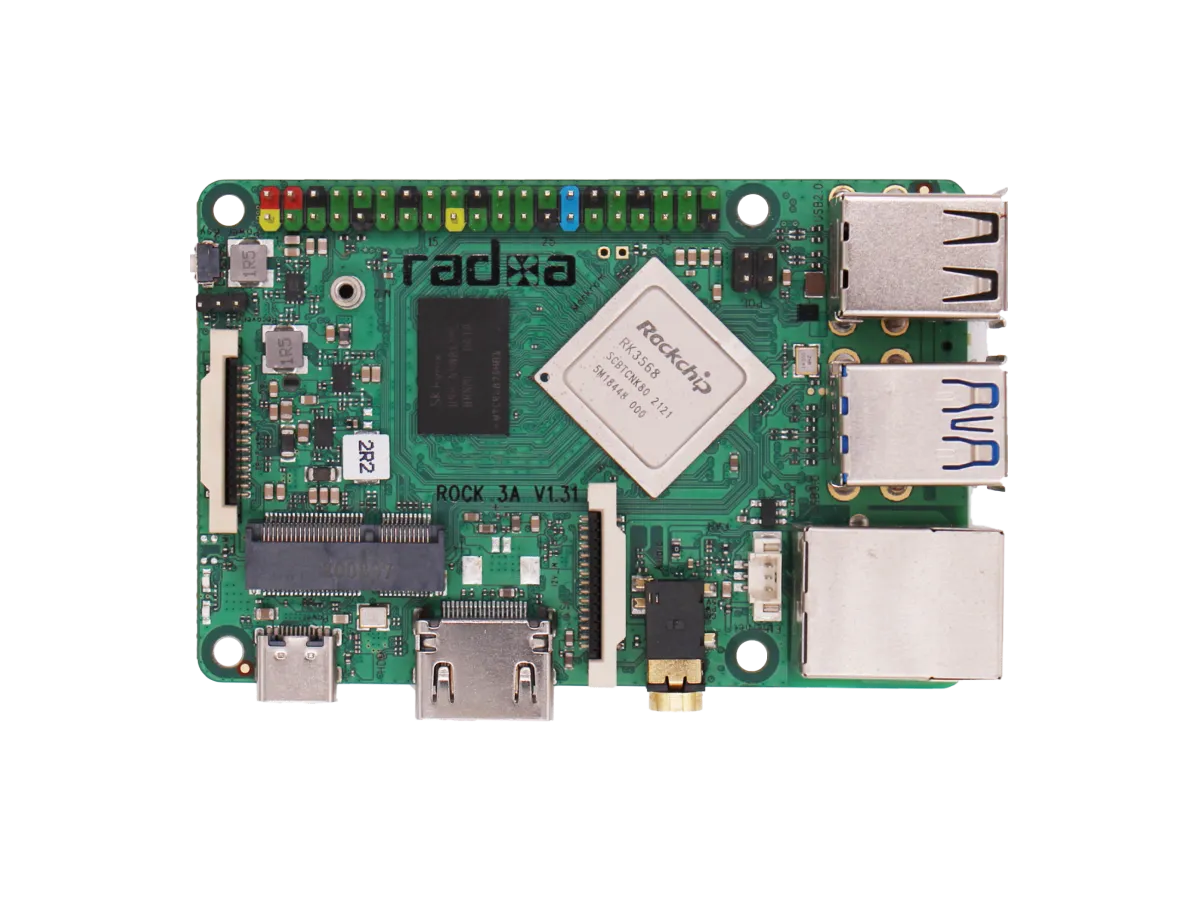
\includegraphics[width=1.0\linewidth]{imagens/rock3a.png}
    \caption{Placa Radxa ROCK 3A}
    \label{fig:rock3a}
\end{figure}

\section{Metodologia}

A metodologia para o desenvolvimento do projeto começou com o planejamento da solução. Para isso, foi necessário quebrar o problema em problemas menores que podem ser resolvidos mais facilmente.

A primeira quebra a ser feita é a separação do problema de leitura de placas de carro do problema do hardware que executará a solução. Primeiro é necessário atingir um resultado satisfatório em ambiente de desenvolvimento para só então evoluir para o ambiente final da prova de conceito.

\subsection{Planejamento do modelo de leitura de placas}

O \textit{input} com o qual a solução irá lidar é uma imagem na qual aparece a placa de um carro. Porém, apenas a placa em si nos interessa, sendo todo o resto da imagem informação desnecessária para o nosso objetivo. Portanto, o primeiro problema consiste em transformar a imagem que contém a placa de um carro em uma imagem que contém \textit{somente} a placa de um carro. Todo o resto deve ser removido.

A partir da imagem da placa do carro, o próximo desafio é identificar onde estão as letras e os números. Modelos de classificação de imagens, principalmente de imagens de caracteres, são extremamente eficazes, mas precisam que a imagem contenha única e exclusivamente o caractere a ser classificado. Dessa forma, a imagem contendo a placa inteira precisa ser quebrada em pedaços, cada um contendo um caractere.

Para que essa divisão da placa em caracteres tenha sucesso, é necessário saber como os caracteres estão dispostos pela placa, o que varia comforme o tipo da placa. No Brasil existem dois de \textit{layout} de placa permitidos: O tipo antigo, ainda em circulação, e o tipo Mercosul, que passou a ser obrigatório para veículos novos no Brasil em 2020.

Por fim, o último problema é classificar cada imagem de caractere. Tendo as imagens classificadas, e sendo a sua ordem na placa conhecida, é possível inferir a placa do veículo. Com isso, o problema do modelo estaria resolvido.

A conclusão é que o problema do modelo de leitura de placas de carro pode ser dividido nos seguintes três problemas:

\begin{itemize}
	\item Detecção e classificação da placa
	\item Extração dos caracteres
	\item Classificação dos caracteres
\end{itemize}

A detecção e classificação são uma única etapa pois modelos de detecção de objetos costumam ter a capacidade de detectar objetos de múltiplas classes e identificar qual é a classe de cada objeto detectado. Isso permite que a detecção da placa e a classificação do tipo de placa sejam feitos de uma só vez.

Para que a extração e classificação dos caracteres funcione bem, é vital que haja um pré-processamento da imagem da placa extraída pela detecção, com objetivo de remover ao máximo o ruído da imagem e deixando-a o mais limpa possível.

O diagrama da figura \ref{fig:pipeline} mostra todas essas etapas assim como sus entradas e saídas.

\begin{figure}[H]
    \centering
    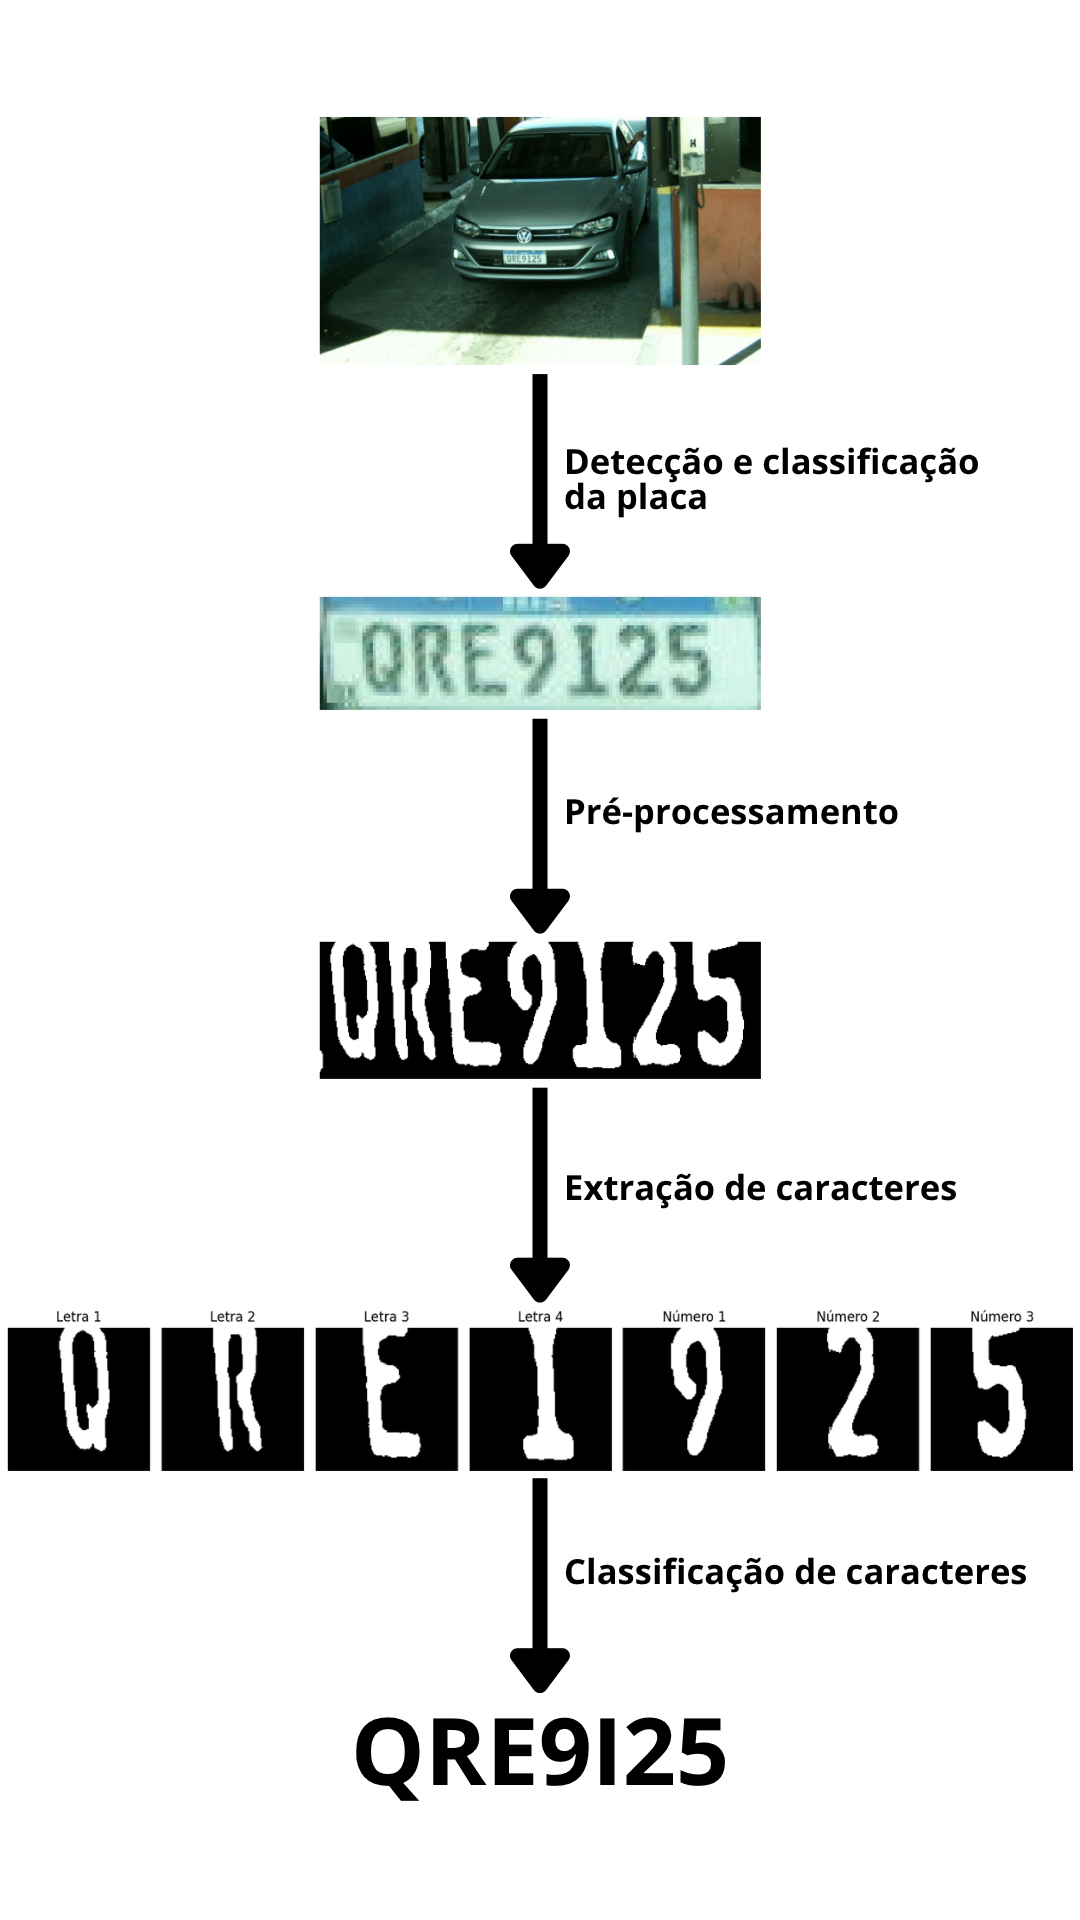
\includegraphics[width=0.5\linewidth]{imagens/diagrama_pipeline.png}
    \caption{Diagrama das etapas da leitura de placas}
    \label{fig:pipeline}
\end{figure}

\subsection{Planejamento da execução dos modelos na placa ROCK 3A}

A placa ROCK 3A é equipada com uma NPU (\textit{Neural Processing Unit}), que em tese executa modelos de redes neurais de forma mais eficiente que uma CPU. Portanto, nosso objetivo é que os modelos sejam executados na NPU.

Para isso são necessárias duas etapas principais: Preparação da placa e preparação dos modelos.

A preparação da placa envolve:

\begin{itemize}
	\item Instalar o sistema operacional
	\item Instalar todo o software necessário para inferência
	\item Ativar a NPU
\end{itemize}

A preparação dos modelos consiste basicamente em convertê-los para o formato RKNN, que é o formato aceito para a NPU do ROCK 3A.

\subsection{Planejamento das etapas do projeto}

Tendo o planejamento do modelo e da execução na placa, podemos agora pensar nas etapas do projeto. Essas etapas devem abarcar o desenvolvimento do modelo, a execução no \textit{hardware} do projeto e o teste final dos resultados.

As etapas sequenciais, portanto são:

\begin{enumerate}
	\item Preparação dos dados a serem utilizados para treinamento e teste do modelo
	\item Treinamento de um modelo de detecção de placas (apenas identifica o tipo e a posição da placa)
	\item Desenvolvimento de um algoritmo de pré-processamento e extração de caracteres
	\item Geração de um dataset de caracteres extraídos
	\item Treinamento de modelos de classificação de caracteres
	\item Conversão dos modelos para formato compatível com NPU
	\item Teste dos modelos no computador e na placa
\end{enumerate}

\subsection{Preparação dos dados}

A preparação inicial dos dados envolveu principalmente dois procedimentos: Separação e organização. 

A separação consistiu em separar os dados em três subgrupos, sendo eles \textbf{treino}, \textbf{validação} e \textbf{teste}. Os subgrupos possuem a função de impedir que dados utilizados no desenvolvimento da solução sejam também utilizados para avaliar a qualidade da mesma, de forma a não gerar um viés nos testes.

A organização, por outro lado, foi feita tendo em mente o algoritmo de treinamento do modelo de detecção de placas, que requer que os dados estejam organizados em uma dada estrutura, como veremos mais à frente. Além disso, o \textit{dataset} de teste foi organizado para os testes da solução completa, a serem realizados no final do projeto.

\subsection{Treinamento do modelo de detecção de placas}

O modelo de detecção de placas possui três funções:

\begin{itemize}
	\item Detectar os limites da placa na imagem (superior, inferior, esquerdo e direito)
	\item Detectar as coordenadas dos quatro cantos da placa
	\item Detectar a classe da placa entre duas possibilidades: Brasil e Mercosul
\end{itemize}

Sendo que a classe "Brasil" refere-se ao modelo antigo de placas brasileiras, enquanto "Mercosul" refere-se ao modelo novo, adotado em todo o bloco Mercosul.

Para essa funcionalidade o método utilizado foi treinar um modelo pré-treinado de detecção de objetos, adaptando-o para a necessidade específica do projeto. A biblioteca Ultralytics, do Python, oferece uma interface para esse tipo de treinamento de modelos de detecção de objetos. Essa interface requer uma organização específica dos dados, que foi realizada na etapa anterior.

\subsection{Desenvolvimento de algorítmo de pré-processamento e extração de caracteres}

O modelo de detecção de placas de carro entrega a posição da placa na imagem e as coordenadas dos quatro cantos. A partir dessa informação é trivial cortar apenas a parte da imagem que contém a placa. Isso já ajuda bastante no processo de extração dos caracteres, mas não é suficiente. Uma questão importante é que em muitos casos a placa possui certa rotação ou perspectiva, o que pode atrapalhar bastante. Para corrigir isso é possível aplicar uma transformação linear combase nas coordenadas dos quatro cantos que corrige essa distorção.

Além disso, as placas possuem partes que não nos interessam. Apenas os caracteres são relevantes para a leitura, sendo todo o resto (parte superior, inferior, laterais) descartável.

Um outro fato importante é que é possível saber previamente quais caracteres são letras e quais são números com base em sua posição na placa. Tanto a placa Brasil quanto a Mercosul possui uma sequência bem definida de letras e números, de forma que basta saber qual é a classe da placa para que se saiba onde as letras e os números estão posicionados.

Com base nesses fatos, o algoritmo de pré-processamento e extração de caracteres deve:

\begin{itemize}
	\item Corrigir a perspectiva e rotação da placa para que ela fique reta e com dimensões padronizadas
	\item Cortar os cantos que não possuem informações relevantes
	\item Fazer uma limpeza e remover todo o ruído desnecessário
	\item Dividir a placa em pedaços, cada um contendo um caractere
	\item Padronizar as dimensões das imagens de caracteres
	\item Separar os caracteres extraídos em letras e números com base na posição
\end{itemize}

\subsection{Geração de um \textit{dataset} de caracteres extraídos}

Para que seja possível treinar os modelos de classificação dos caracteres é necessário criar um \textit{dataset} de caracteres. Tendo sido realizadas as etapas anteriores, basta aplicar a detecção de placa e extração de caracteres em cada imagem dos dados de treinamento para criar um \textit{dataset} de caracteres. Como sabemos previamente quais placas são do tipo Brasil e quais são Mercosul, assim como também sabemos quais caracteres são números e quais são letras, é possível criar \textit{datasets} separados para cada categoria, resultando em quatro \textit{datasets}:

\begin{itemize}
	\item Números Brasil
	\item Letras Brasil
	\item Números Mercosul
	\item Letras Mercosul
\end{itemize}

Sendo que cada um destes ainda é separado em treino e validação.

\subsection{Treinamento de modelos de classificação de caracteres}

Com o \textit{dataset} de caracteres pronto, basta criar uma arquitetura de modelo de visão computacional e treiná-lo com esses dados. Como os dados já vêm pré-processados e a tarefa de classificação de caracteres não é particularmente complexa, basta uma arquitetura simples de redes neurais convolucionais para resolver esse problema.

\subsection{Conversão dos modelos para formato compatível com NPU}

O formato compatível com a NPU do ROCK 3A é o formato RKNN. A prória documentação da placa indica uma biblioteca chamada \textit{rknn toolkit} que oferece a \textit{API} tanto para conversão dos modelos para esse formato quanto para inferência com esses modelos. Porém, a conversão não é tão trivial, pois precisa ser feita em um ambiente \textit{linux} de uma determinada distribuição e versão. Além disso, os modelos precisam ser exportados para o formato ONNX antes de serem convertidos, pois o \textit{rknn toolkit} faz a conversão entre esses dois formatos.

Além desses requisitos obrigatórios para a conversão, existe um requisito opcional, porém recomendado. Este é que durante a conversão para RKNN os modelos sejam quantizados para \textit{uint8}, ou seja, que seus pessos sejam convertidos de números reais do tipo \textit{float} de 32 \textit{bits} para números inteiros positivos de 8 \textit{bits}. Isso é recomendado pois intensifica a performance da NPU.

Para a quantização é necessário criar um \textit{dataset} de quantização. Esse \textit{dataset} só precisa conter dados de entrada, não sendo necessários os rótulos.

\subsection{Teste dos modelos no computador e na placa}

Uma vez que os modelos estão prontos e convertidos é possível testá-los tanto no computador quanto na placa. No computador ainda é possível testá-los na CPU e na GPU. Para avaliar a performance nos diferentes cenários, vamos usar o \textit{dataset} de teste que foi gerado no começo e avaliar em quantas imagens o modelo acerta a placa do carro.

Porém, a principal diferença entre os locais de execução não deve vir no percentual de acerto, e sim no tempo de inferência. Portanto, é necessário medir o tempo, tanto do modelo de detecção de placa quanto nos modelos de classificação de caracteres.